%%%%%%%%%%%%%%%%%%%%%%%%%%%%%%%%%%%%%%%%%%%%%%%%%%%%%%%%%%%%%%%%%%%%%%%%%%%%%%%%%%
\begin{frame}[fragile]\frametitle{}

\begin{center}
{\Large Topic Modeling}
\end{center}
\end{frame}

%%%%%%%%%%%%%%%%%%%%%%%%%%%%%%%%%%%%%%%%%%%%%%%%%%%%%%%%%%%%%%%%%%%%%%%%%%%%%%%%%%
\begin{frame}[fragile]\frametitle{What is Topic Modeling?}
  \begin{itemize}
  	\item Topic modeling is a form of text mining, a way of identifying patterns in a corpus. 
	\item  You take your corpus and run it through a tool which groups words across the corpus into `topics' ( clusters of words) by a process of similarity.
	\item In a good topic model, the words in topic make sense, for example ``navy, ship, captain'' and ``tobacco, farm, crops.''
  \end{itemize}
\begin{center}
\includegraphics[width=0.6\linewidth,keepaspectratio]{top}
\end{center}
\end{frame}

%%%%%%%%%%%%%%%%%%%%%%%%%%%%%%%%%%%%%%%%%%%%%%%%%%%%%%%%%%%%%%%%%%%%%%%%%%%%%%%%%%
\begin{frame}[fragile]\frametitle{Core Concept: Similarity}
Are these statements similar?
  \begin{itemize}
  	\item ``A seven-year quest to collect samples from the solar system's formation ended in triumph in a dark and wet Utah desert this weekend.''
	\item ``For a month, a huge storm with massive lightning has been raging on Jupiter under the watchful eye of an orbiting spacecraft.''
	\item ``One of Saturn's moons is spewing a giant plume of water vapour that is feeding the planet's rings, scientists say.''
  \end{itemize}
How would you quantify their similarity? How would you decide that two are more similar to each other than to the third? 

\end{frame}

%%%%%%%%%%%%%%%%%%%%%%%%%%%%%%%%%%%%%%%%%%%%%%%%%%%%%%%%%%%%%%%%%%%%%%%%%%%%%%%%%%
\begin{frame}[fragile]\frametitle{Semantic Similarity}
  \begin{itemize}
  	\item A study done in Australia in 2005 : what a sample of Australian college students think is similar. 
	\item Students read hundreds of paired short excerpts from news articles and ranked the pairwise similarity on a scale. 	
	\item Then examined all the classifications, and found that they had a correlation of 0.6. 
	\item That's obviously a positive correlation, but not terribly high. 
	\item So, humans doesn't necessarily agree with each other about semantic similarity
	\item It's kind of a fuzzy notion
  \end{itemize}
\end{frame}

%%%%%%%%%%%%%%%%%%%%%%%%%%%%%%%%%%%%%%%%%%%%%%%%%%%%%%%%%%%%%%%%%%%%%%%%%%%%%%%%%%
\begin{frame}[fragile]\frametitle{Semantic Similarity: Any number?}
  \begin{itemize}
  	\item The study mentioned found that a particular topic modelling technique called latent semantic analysis (LSA) could achieve also a 0.6 correlation with the human ratings
	\item Correlating with the study participant's choice about as well as they correlated with each other.
  \end{itemize}
\end{frame}

%%%%%%%%%%%%%%%%%%%%%%%%%%%%%%%%%%%%%%%%%%%%%%%%%%%%%%%%%%%%%%%%%%%%%%%%%%%%%%%%%%
\begin{frame}[fragile]\frametitle{Who cares about semantic similarity? }
Some use cases:

  \begin{itemize}
  	\item Query large collections of text: Traditionally used on large document collections. Legal discovery. Answer questions or aid searching huge corpora like government regulations, manuals, patent databases, etc.

  	\item  Automatic metadata: system can intelligently suggest tags and categories for documents based on other documents they're similar too. 
  	\item  Recommendations: plagiarism detection, exam scoring. And there are a number of other use cases. 
  	\item  Better human-computer interaction: Matching on similarity rather than words or with regexes allows us to accept broader ranges of input, in theory. 

  \end{itemize}
\end{frame}

%%%%%%%%%%%%%%%%%%%%%%%%%%%%%%%%%%%%%%%%%%%%%%%%%%%%%%%%%%%%%%%%%%%%%%%%%%%%%%%%%%
\begin{frame}[fragile]\frametitle{What is Topic Modeling?}
  \begin{itemize}
  	\item Topic modelling attempts to uncover the underlying semantic structure of text (or other data) by using statistical techniques to identify abstract, recurring patterns of terms in a set of data. 
  	\item These patterns are called topics. They may or may not correspond to our intuitive notion of a topic. 
	\item Topic modelling models documents as collections of features, representing the documents as long vectors that indicate the presence/absence of important features, for example, the presence or absence of words in a document. 
	\item We can use those vectors to create spaces and plot the locations of documents in those spaces and use that as a kind of proxy for their meaning.
  \end{itemize}
\end{frame}

%%%%%%%%%%%%%%%%%%%%%%%%%%%%%%%%%%%%%%%%%%%%%%%%%%%%%%%%%%%%%%%%%%%%%%%%%%%%%%%%%%
\begin{frame}[fragile]\frametitle{What is Topic Modeling?}
  \begin{itemize}
  	\item Topic modeling is an unsupervised algorithm.
  	\item One of the key ideas behind it is that every topic is present to
varying degrees within each document. 
\item The typical output of running a corpus
through TM is a set of distinctive words for each topic and for each document
a percentage value indicating the presence of each topic within that document.
  	\item One of the popular algorithms underlying TM is called Latent Dirichlet Allocation (LDA) and
was described in a paper published by Blei, Ng and Jordan in 2003. 
  \end{itemize}
\end{frame}

%%%%%%%%%%%%%%%%%%%%%%%%%%%%%%%%%%%%%%%%%%%%%%%%%%%%%%%%%%%%%%%%%%%%%%%%%%%%%%%%%%
\begin{frame}[fragile]\frametitle{What Topic Modeling is NOT?}
Topic modelling: 
  \begin{itemize}
  	\item Does not parse sentences. 
  	\item In fact, knows nothing about word order. 
  	\item Makes no attempt to ``understand'' grammar or language syntax. 
  \end{itemize}
\end{frame}

%%%%%%%%%%%%%%%%%%%%%%%%%%%%%%%%%%%%%%%%%%%%%%%%%%%%%%%%%%%%%%%%%%%%%%%%%%%%%%%%%%
\begin{frame}[fragile]\frametitle{How does it work?}
Manual mode:
  \begin{itemize}
  	\item Imagine working through an article with a set of highlighters
	\item A different color for the key words of themes within the paper as you come across them
	\item Once done, you could copy out the words as grouped by the color you assigned them. That list of words is a topic, and each color represents a different topic.
	\item The popular LDA which is used to extract topics is based on ``Dirichlet Distribution''.
	\item Trying to understand LDA (and its proof) is not trivial (so leave it!!)
  \end{itemize}
\end{frame}

%%%%%%%%%%%%%%%%%%%%%%%%%%%%%%%%%%%%%%%%%%%%%%%%%%%%%%%%%%%%%%%%%%%%%%%%%%%%%%%%%%
\begin{frame}[fragile]\frametitle{Still, how does it work?}
  \begin{itemize}
  	\item Each document contains a mixture of different topics.
	\item  ``topic'' can be understood as a collection of words that have different probabilities of appearance. 
	\item One topic might contain many occurrences of ``organize,'' ``committee,'' ``direct,'' and ``lead.'' 
	\item Another might contain a lot of ``mercury'' and ``arsenic,'' with a few occurrences of ``lead.'' 
%	\item Most of the occurrences of ``lead'' in this second topic, incidentally, are nouns instead of verbs; 
%	\item LDA will be that it implicitly sorts out the different contexts/meanings (PoS).
  \end{itemize}
\begin{center}
\includegraphics[width=0.4\linewidth,keepaspectratio]{top1}
\end{center}
\end{frame}

%%%%%%%%%%%%%%%%%%%%%%%%%%%%%%%%%%%%%%%%%%%%%%%%%%%%%%%%%%%%%%%%%%%%%%%%%%%%%%%%%%
\begin{frame}[fragile]\frametitle{Still, how does it work?}
  \begin{itemize}
  	\item Can't directly observe topics; what we have are documents
	\item Topic modeling is a way of extrapolating backward to infer the discourses (``topics'') that could have generated them.
%	\item Unfortunately, there is no way to infer the topics exactly: there are too many unknowns. 
%	\item But pretend for a moment that we had the problem mostly solved. 
%	\item Suppose we knew which topic produced every word in the collection, except for this one word in document D. 
%	\item The word happens to be ``lead,'' which we'll call word type W. 
	\item How are we going to decide whether this occurrence of W belongs to topic Z?
%  \end{itemize}
%\end{frame}
%
%%%%%%%%%%%%%%%%%%%%%%%%%%%%%%%%%%%%%%%%%%%%%%%%%%%%%%%%%%%%%%%%%%%%%%%%%%%%%%%%%%%
%\begin{frame}[fragile]\frametitle{Still, how does it work?}
%  \begin{itemize}
%  	\item We can't know for sure.
	\item But one way to guess is to consider two questions.
	  \begin{itemize}
	\item How often does ``lead'' appear in topic Z? 
	\item How common is topic Z in the rest of this document? 
	  \end{itemize}
	\item We will find probability of W present in Z for this document D, as follows:
\begin{center}
\includegraphics[width=0.8\linewidth,keepaspectratio]{top2}
\end{center}
	\item Its is calculated by multiplying the frequency of this word type W in Z by the number of other words in document D that already belong to Z. 
  \end{itemize}
\end{frame}

%%%%%%%%%%%%%%%%%%%%%%%%%%%%%%%%%%%%%%%%%%%%%%%%%%%%%%%%%%%%%%%%%%%%%%%%%%%%%%%%%%
\begin{frame}[fragile]\frametitle{Document generation}

Document is generated using some settings. Which set of settings (machine 1 or machine 2) are more similar to the real document?

\begin{center}
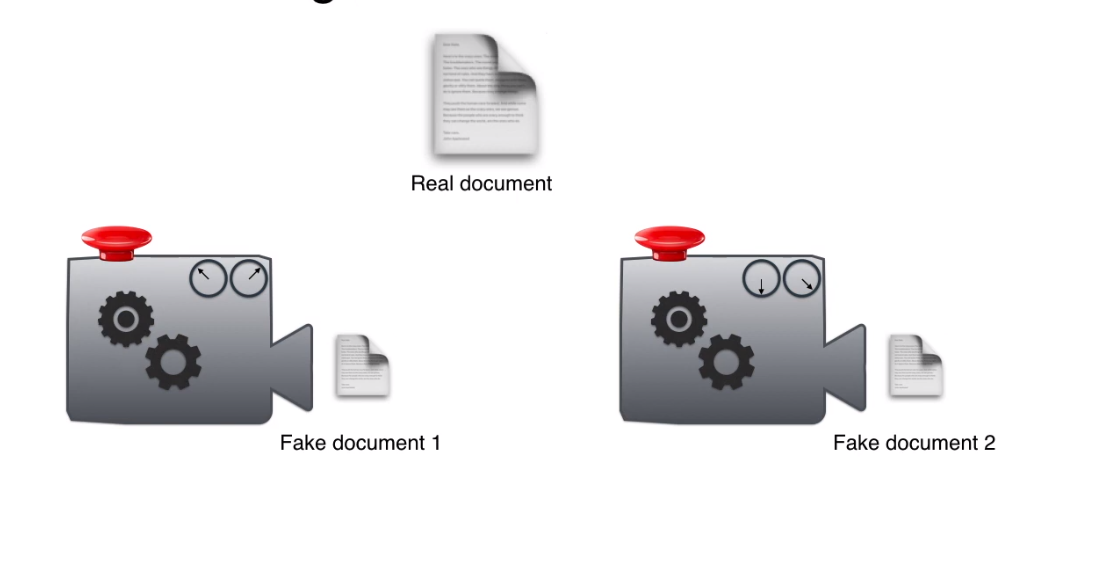
\includegraphics[width=0.9\linewidth,keepaspectratio]{lda2}
\end{center}

{\tiny (Ref: Natural Language Processing - Luis Serrano)}
\end{frame}


%%%%%%%%%%%%%%%%%%%%%%%%%%%%%%%%%%%%%%%%%%%%%%%%%%%%%%%%%%%%%%%%%%%%%%%%%%%%%%%%%%
\begin{frame}[fragile]\frametitle{Settings in generator machines}

Settings are nothing but two Dirichlet Distributions (doc to topic and topic to words) and then two multinomial distributions (doc to topic and topic to words).

\begin{center}
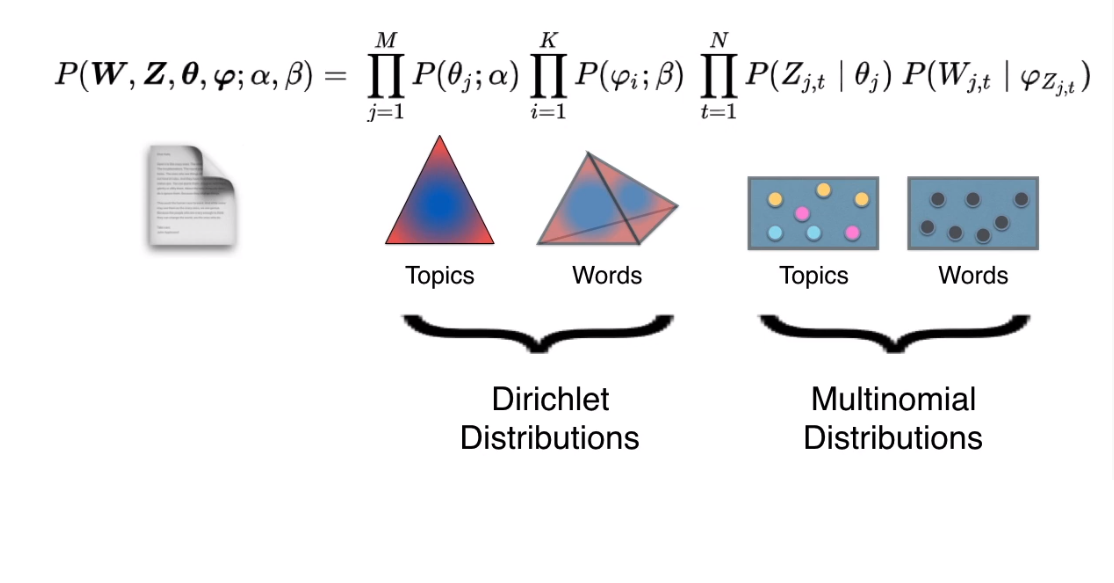
\includegraphics[width=0.9\linewidth,keepaspectratio]{lda3}
\end{center}

(Note: for 4 words, square is not chosen for Dirichlet distribution as its diagonal points are not equidistant, so tetrahedron is chosen)


{\tiny (Ref: Natural Language Processing - Luis Serrano)}
\end{frame}

%%%%%%%%%%%%%%%%%%%%%%%%%%%%%%%%%%%%%%%%%%%%%%%%%%%%%%%%%%%%%%%%%%%%%%%%%%%%%%%%%%
\begin{frame}[fragile]\frametitle{Example generation}

Example document is generated.

\begin{center}
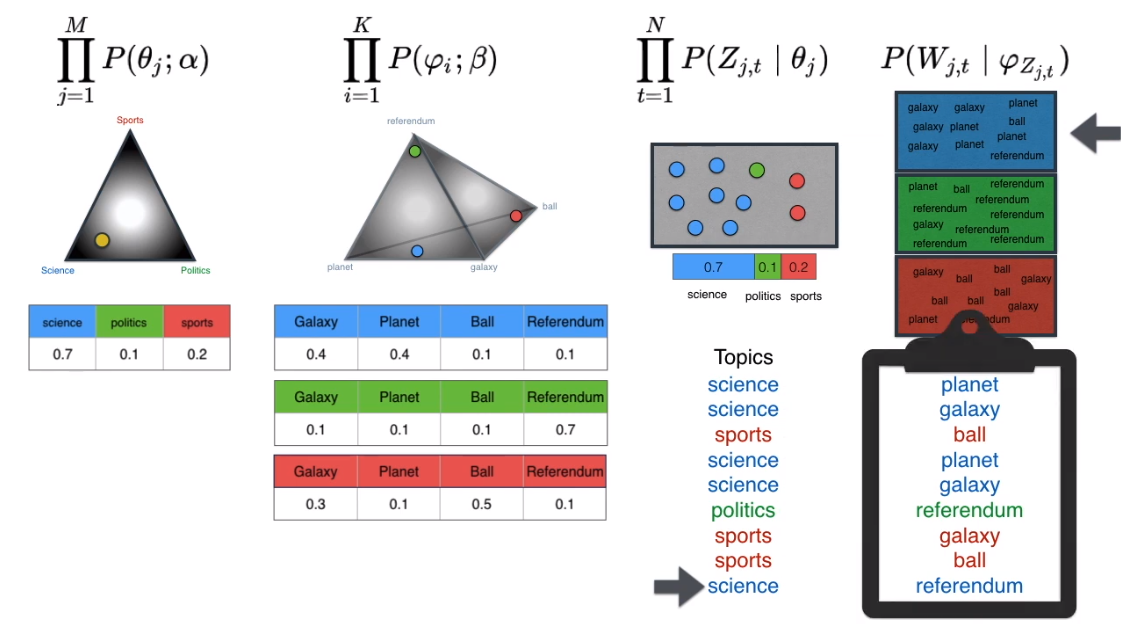
\includegraphics[width=0.9\linewidth,keepaspectratio]{lda1}
\end{center}

{\tiny (Ref: Natural Language Processing - Luis Serrano)}
\end{frame}

%%%%%%%%%%%%%%%%%%%%%%%%%%%%%%%%%%%%%%%%%%%%%%%%%%%%%%%%%%%%%%%%%%%%%%%%%%%%%%%%%%
\begin{frame}[fragile]\frametitle{Example generation}

Multiple sample documents are generated and checked against the real ones.

\begin{center}
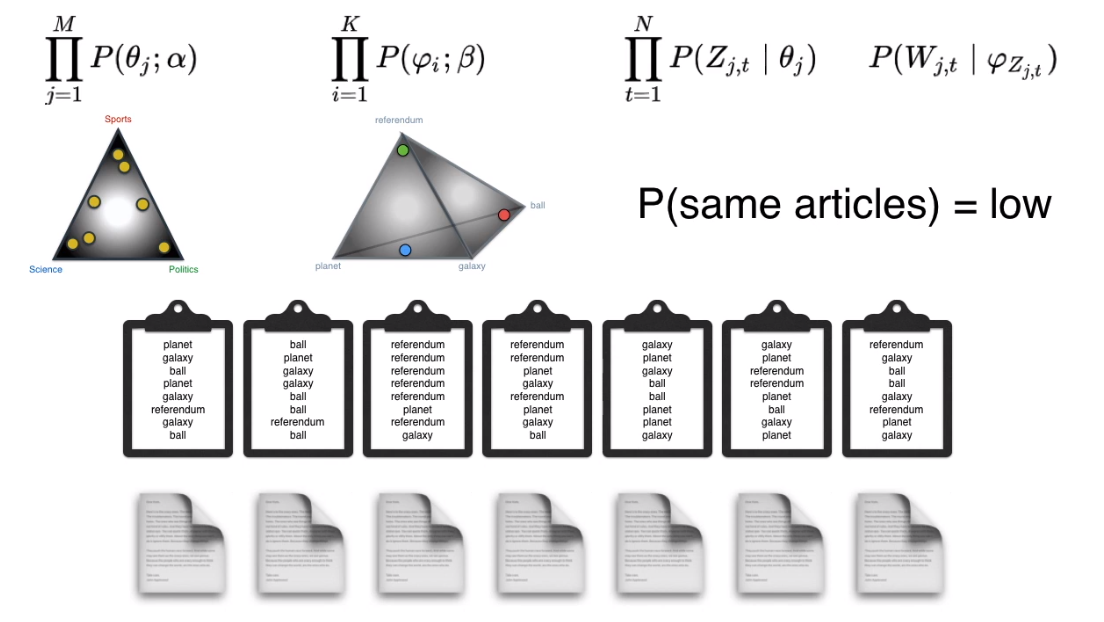
\includegraphics[width=0.9\linewidth,keepaspectratio]{lda4}
\end{center}

The settings which give original artical back, ie with better probability are chosen.

{\tiny (Ref: Natural Language Processing - Luis Serrano)}
\end{frame}



%%%%%%%%%%%%%%%%%%%%%%%%%%%%%%%%%%%%%%%%%%%%%%%%%%%%%%%%%%%%%%%%%%%%%%%%%%%%%%%%%%%
%\begin{frame}[fragile]\frametitle{Still, how does it work?}
%  \begin{itemize}
%  	\item If we had a wild strategy we would have gone to docouemtns, word by word, and assigned each to some random topic word. Bad, right?
%	\item Instead, we could go through the collection, word by word, and reassign each word to a topic, guided by the formula. Somewhat better, right?
%	\item As we do that, words will gradually become more common in topics where they are already common.
%	\item And also, topics will become more common in documents where they are already common.
%	\item Thus our model will gradually become more consistent as topics focus on specific words and documents.
%  \end{itemize}
%\end{frame}

%%%%%%%%%%%%%%%%%%%%%%%%%%%%%%%%%%%%%%%%%%%%%%%%%%%%%%%%%%%%%%%%%%%%%%%%%%%%%%%%%%
\begin{frame}[fragile]\frametitle{Practically}
  \begin{itemize}
%  	\item You assign words to topics randomly and then just keep improving the model, to make your guess more internally consistent, until the model reaches an equilibrium that is as consistent as the collection allows. 
	\item Topic modeling gives us a way to infer the latent structure behind a collection of documents.
	\item David Blei invented LDA, and writes well, so if you want to understand why this technique has ``Dirichlet'' in its name, his works are the next things to read
  \end{itemize}
\end{frame}
%%%%%%%%%%%%%%%%%%%%%%%%%%%%%%%%%%%%%%%%%%%%%%%%%%%%%%%%%%%%%%%%%%%%%%%%%%%%%%%%%%
\begin{frame}[fragile]\frametitle{How Topics look?}
\begin{lstlisting}
>>> lsi_model.show_topics()
'-0.203*"smith" + 0.166*"jan" + 0.132*"soccer" + 0.132*"software" + 0.119*"fort" + -0.119*"nov" + 0.116*"miss" + -0.114*"opera" + -0.112*"oct" + -0.105*"water"',

'0.179*"squadron" + 0.158*"smith" + -0.140*"creek" + 0.135*"chess" + -0.130*"air" + 0.128*"en" + -0.122*"nov" + -0.120*"fr" + 0.119*"jan" + -0.115*"wales"', 

'0.373*"jan" + -0.236*"chess" + -0.234*"nov" + -0.208*"oct" + 0.151*"dec" + -0.106*"pennsylvania" + 0.096*"view" + -0.092*"fort" + -0.091*"feb" + -0.090*"engineering"',
\end{lstlisting}
  \begin{itemize}
  	\item These three abbreviated topics were extracted from a large corpora of texts by gensim.
	\item Words are not ordered.
	\item Positive and negative weights for each word, which get smaller in magnitude as the topic goes on. 

  \end{itemize}
\end{frame}

%%%%%%%%%%%%%%%%%%%%%%%%%%%%%%%%%%%%%%%%%%%%%%%%%%%%%%%%%%%%%%%%%%%%%%%%%%%%%%%%%%
\begin{frame}[fragile]\frametitle{Example}
Suppose you have the following set of sentences:
  \begin{itemize}
  	\item     I eat fish and vegetables.
  	\item         Fish are pets.
  	\item         My kitten eats fish.
  \end{itemize}
Latent Dirichlet allocation (LDA) is a technique that automatically discovers topics that these documents contain.

LDA achieves the above results in 3 steps. Instead of sentences, imagine you have 2 documents with the following words (cleaned docs):
\begin{center}
\includegraphics[width=0.5\linewidth,keepaspectratio]{top3}
\end{center}
\end{frame}

%%%%%%%%%%%%%%%%%%%%%%%%%%%%%%%%%%%%%%%%%%%%%%%%%%%%%%%%%%%%%%%%%%%%%%%%%%%%%%%%%%
\begin{frame}[fragile]\frametitle{Algorithm}
  \begin{itemize}
  	\item    Step 1: You tell the algorithm how many topics you think there are.Its just a number. Then topics would have ID's like Topic1, Topic2, etc.
  	\item    Step 2: Assign every word to a temporary topic.
  	  \begin{lstlisting}
  			 Topic1    Topic2    Topic3
word1    	1       		0     		36
Word2   	6       		3      		2
:

    			Topic1     Topic2   	 Topic3
doc1		25	          2               11
doc2		3             7               34
:
\end{lstlisting}
	\item Step 3: In iteration, for each doc, for each word, its topic assignment is updated based on two criteria:
      \begin{itemize}
  	\item   How prevalent is that word across topics?
    	\item How prevalent are topics in the document?
  \end{itemize}
  \end{itemize}
\end{frame}


%%%%%%%%%%%%%%%%%%%%%%%%%%%%%%%%%%%%%%%%%%%%%%%%%%%%%%%%%%%%%%%%%%%%%%%%%%%%%%%%%%
\begin{frame}[fragile]\frametitle{Example}
  \begin{itemize}
	\item Following shows two documents X and Y, and number of topics to be be generated is 2.
	\item Lets call them Topics F (for Food) and P (for Pets)
	\item Go to every document and for each word write its Topic ID, RANDOMLY.
\item Say, starting with first word of Doc Y: ``fish'' in Doc Y.
\item Rest all the topic-word-docs assignments, although RANDOM are ASSUMED to be correct (this method/sampling is called Gibb's sampling)
  \end{itemize}
\begin{center}
\includegraphics[width=0.5\linewidth,keepaspectratio]{top4}
\end{center}

\end{frame}

%%%%%%%%%%%%%%%%%%%%%%%%%%%%%%%%%%%%%%%%%%%%%%%%%%%%%%%%%%%%%%%%%%%%%%%%%%%%%%%%%%
\begin{frame}[fragile]\frametitle{How prevalent is that word across topics? }
  \begin{itemize}
	\item In Doc X, ``fish'' is with TopicF in both the cases, ie 2/2. It is with TopicP 0 times.
	\item In (remaining) Doc Y, ``fish'' is with TopicF in 1 case, ie 1/1. It is with TopicP 0 times.
	\item Total: ``fish'' with TopicF 3/3 times and with TopcP 0 times.
  \end{itemize}
  
%Since ``fish'' words across both documents nearly half of remaining Topic F words but 0\% of remaining Topic P words, a ``fish'' word picked at random would more likely be about Topic F.
\begin{center}
\includegraphics[width=0.5\linewidth,keepaspectratio]{top5}

\includegraphics[width=0.5\linewidth,keepaspectratio]{word39}
\end{center}
\end{frame}




%%%%%%%%%%%%%%%%%%%%%%%%%%%%%%%%%%%%%%%%%%%%%%%%%%%%%%%%%%%%%%%%%%%%%%%%%%%%%%%%%%
\begin{frame}[fragile]\frametitle{How prevalent are topics in the document?}

  \begin{itemize}
  	\item Now within the single document, ie Doc Y, how are topics distributed?
	\item 2 TopicFs, 2 TopicPs. 50-50\%
	\item So, their length bars are equal (but vertical!!)
  \end{itemize}
%Since the words in Doc Y are assigned to Topic F and Topic P in a 50-50 ratio, the remaining ``fish'' word seems equally likely to be about either topic.
\begin{center}
\includegraphics[width=0.5\linewidth,keepaspectratio]{top6}

\includegraphics[width=0.5\linewidth,keepaspectratio]{top10}
\end{center}


\end{frame}

%%%%%%%%%%%%%%%%%%%%%%%%%%%%%%%%%%%%%%%%%%%%%%%%%%%%%%%%%%%%%%%%%%%%%%%%%%%%%%%%%%
\begin{frame}[fragile]\frametitle{Probability of Assignment }
  \begin{itemize}
	\item Multiply horizontal and vertical lengths, get get areas
	
\begin{center}
\includegraphics[width=0.5\linewidth,keepaspectratio]{top11}
\end{center}
\item Topic1 has more area, so ``fish'' going to TopcF is proportionally more
\item Go back and update the assignment value of ``fish'' to have more in TopicF. 
\item Repeating this `n' iterations, words cluster to topics and topics cluster to documents.
  \end{itemize}
  
%Since ``fish'' words across both documents nearly half of remaining Topic F words but 0\% of remaining Topic P words, a ``fish'' word picked at random would more likely be about Topic F.
\end{frame}

%%%%%%%%%%%%%%%%%%%%%%%%%%%%%%%%%%%%%%%%%%%%%%%%%%%%%%%%%%%%%%%%%%%%%%%%%%%%%%%%%%
\begin{frame}[fragile]\frametitle{Interesting fact}

  \begin{itemize}
	\item Even though value for TopicP was 0, we did not show the bar length to be 0, but some value.
	\item They are hyper parameters, one in each dimension, alpha and beta. (go back to probability formulation)
	\item alpha is for value adding to word-topics say 0.8 as smoothing constant
	\item beta is for value added to doc=topics likings
  \end{itemize}
  
%Since ``fish'' words across both documents nearly half of remaining Topic F words but 0\% of remaining Topic P words, a ``fish'' word picked at random would more likely be about Topic F.
\end{frame}
%%%%%%%%%%%%%%%%%%%%%%%%%%%%%%%%%%%%%%%%%%%%%%%%%%%%%%%%%%%%%%%%%%%%%%%%%%%%%%%%%%
\begin{frame}[fragile]\frametitle{Results}
  \begin{itemize}
	\item In conclusion, we would assign the ``fish'' word of Doc Y to Topic F. Go to next word (assume remaining assignments are perfect)
  	\item   The process of checking topic assignment is repeated for each word in every document, cycling through the entire collection of documents multiple times. 
	\item This iterative updating is the key feature of LDA that generates a final solution with coherent topics.
  \end{itemize}
\end{frame}



%%%%%%%%%%%%%%%%%%%%%%%%%%%%%%%%%%%%%%%%%%%%%%%%%%%%%%%%%%%%%%%%%%%%%%%%%%%%%%%%%%%
%\begin{frame}[fragile]\frametitle{LSA}
%  \begin{itemize}
%  	\item LSI uses a technique called singular value decomposition (SVD) to reduce the original term/document matrix's number of dimensions and keep the most information for a given number of topics. 
%  	\item  SVD decomposes a matrix into three simpler matrices 
%  	\item  Full rank SVD would be able to recreate the underlying matrix exactly from those three matrices
%  	\item  Lower-rank SVD provides the best (least square error) approximation of the matrix 
%  	\item  This approximation can find interesting relationships among data
%  	\item  It preserves most information while reducing noise and merging dimensions associated with terms that have similar meanings
%  \end{itemize}
%\end{frame}


